\subsection{Quantitative Data}

    %What the data said

    This section presents the results from the two workshops held, in form of lessons learned. Also, some of the quiz results are shown.

    \subsubsection{Quiz Results from the Coaches}

    Quiz results ranges from the worst on 24\% (getting 4/17 correct answers) to 100\% (which has happened on 52/101 instances, for all of the quizzes). Week 9 was undoubtably the hardest quiz, with the topic being "Goal Setting and Action Plan" (17 questions, average being 76.22\% correct answers, 18 quiz results submitted). The easiest quizzes are week 3 "Financial literacy" (11 questions), week 6 "Mastering sales" (9 questions) and week 7 "Sales day" (3 questions), where all of the results are 100\%.

    There are some amount of coaches that have taken the same quizzes multiple times. From this, interesting conclusions can be drawn. Attending the lecture shows a 15.0\% average increase in quiz results, compared to an 12.8\% increase with simply taking the quiz two times. This shows that a lecture is still more effective than learning via the app.

    Time to finish a quiz took between 2 minutes to 33 minutes (3/4 quizzes that took longer than 25 minutes were on quiz 9, there is a correlation with number of questions). Most of the quizzes took under 5 minutes to complete, and results are always over 80\% for these instances. This shows that the coach had a high confidence with the answers. Similarly, all of the scores under 60\% has taken more than 20 minutes. This can be explained by that the coach is unfamiliar with the app or smartphone, and that the coach is uncertain of the answers.

    It is seen in the quiz results that the quizzes did get gradually more challenging, as the average of quiz scores gets lower after day 3 of training, when it was discovered was welcoming the quizzes to get harder.

    The quiz scores when quizzes are performed in group is very varying (from 24\% to 100\%), and it is observed that influence of another coach can lead both to a worse score than their individual average, and a higher score. It is interesting to see that the three coaches that have the worst average (67, 72 and 85\%) are also the ones that have taken quizzes the least times individually, and the most taking quizzes together with others. This may show that the app is more effective when used individually, and there seem no other connection to previous entrepreneurial activity or background.

    There are few correlations that can be made between the coach's background and experience, compared with quiz results or app behavior. Nothing in the coach information distinguishes the worst 3 performers in the quiz. For the opposite, there is however a noticable behaviour that being confident, having trained youth, leadership experience, business experience, care for community, care for oneself and confidence to take on many youth, almost guarantees a high quiz average (which demonstrates learning) and quizzes done (which demonstrates motivation).

    For coaches with 0-1 negative remarks during the interviews (n=6) compared to coaches with 2-4 negative remarks (n=4), their quiz average is but 2\% higher (87\% to 85\%). This is not significant, but this number is increased to 93\% (an 8\% increase) if the outlier from the group is removed (a coach which only did three quizzes with average of 57\%). In the future, more research could be done into comparing coach data with quiz results.

    %Comparing instances when coaches have taken a test before and after a lecture, the results are: 71\%to 100\%, 59\% to 74\%, 80\% to 86\%, 90\% to 100\%. Without the lecture, improvements has been from 80 to 90, 100 to 100 to 100, 90 to 90, 80 to 100, 90 to 100, 100 to 100, 86 to 100, 100 to 100, 90 to 100.

    \subsubsection{Lessons Learned from Unbiased App Design by Coaches: Use Case 1}

    The result was fantastic, in the sense that it gave an unbiased look at what the coaches expected from the app, what functionality wasn't important, and into their technical preferences. A simpler design than originally thought was deemed sufficient, and the simple sketches guided continued development of the app during the week. From using the devices, it was found that most coaches prefer using the tablet (5 for tablet, versus 2 for smartphone and 2 for computer). Both the designs and insights gained were used throughout the week to further improve the simple app created at the end of iteration 1. The workshop gave great insights to who the coaches were and their thinking. \todo{Add image here}

    \subsubsection{Lessons Learned from Unbiased App Design by Coaches: Use Case 2}

    During this workshop, the focus was to examine what builds confidence among the coaches. The following clusters could be determined: "I believe in myself" (3 coaches), "I believe in God" (2 coaches), "I am well prepared" (4 coaches) and "I am certified" (1 coach). See figure \ref{fig:zambiaWorkshop2} for the different clusters.

    \todo{Make full-page}
    \begin{figure}[h]
        \centering
        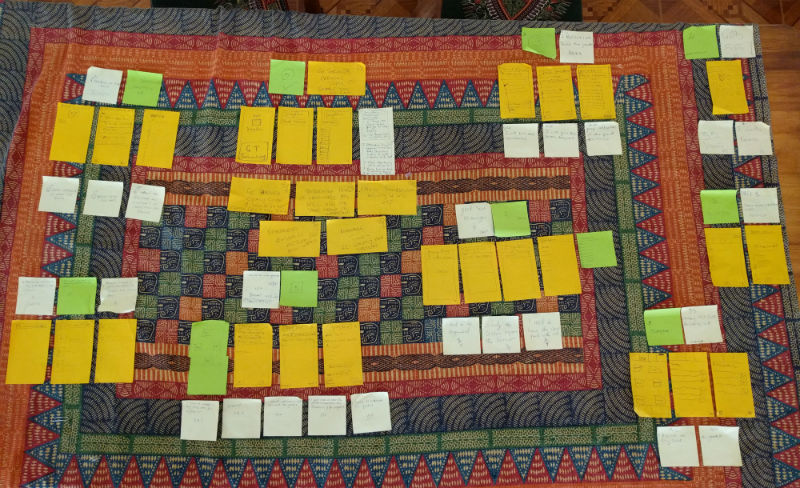
\includegraphics[width=0.7\textwidth]{zambiaWorkshop2small.jpg}
        \caption{The clustered postits with needs, together with included design proposals.}
        \label{fig:iteration}
    \end{figure}

    Josefina comments after the workshop: “I have a problem: There is no way I can control them how they have prepared themselves for a youth session.", says Josefina.
